%% Slides for ".NET Programming" by Chunyu Wang <chunyu@hit.edu.cn> %%

\section{多线程}

% http://msdn2.microsoft.com/zh-cn/library/system.threading.aspx

\begin{frame}
\frametitle{多线程(\textit{Multithreading})}
\begin{block}{\textit{Thread}}
  \CJKindent 线程本质上是一个独立运行的代码段,是操作系统分配处理器时间的基本单元,.NET 中的线程实际
  是操作系统线程的包装器,由操作系统创建和运行。
\end{block}
\begin{itemize}
\item 使用线程,可以提高性能,将任务分解在多个线程中
\item 提高响应能力,如在通过网络发送文件时,接受键盘输入
\item 方便移植到多处理器的计算机上
\end{itemize}
\medskip
\begin{itemize}
\item 程序稍复杂,需要启动、监视、等待线程结束等
\item 多线程使用同一资源,需要进行同步,可能发生死锁
\item 多线程的控制需要一定的处理器时间
\end{itemize}
\end{frame}

\begin{frame}
\frametitle{线程的状态}
\begin{itemize}
\item 运行中的线程有几种不同状态
\end{itemize}
\begin{figure}
  \centering
  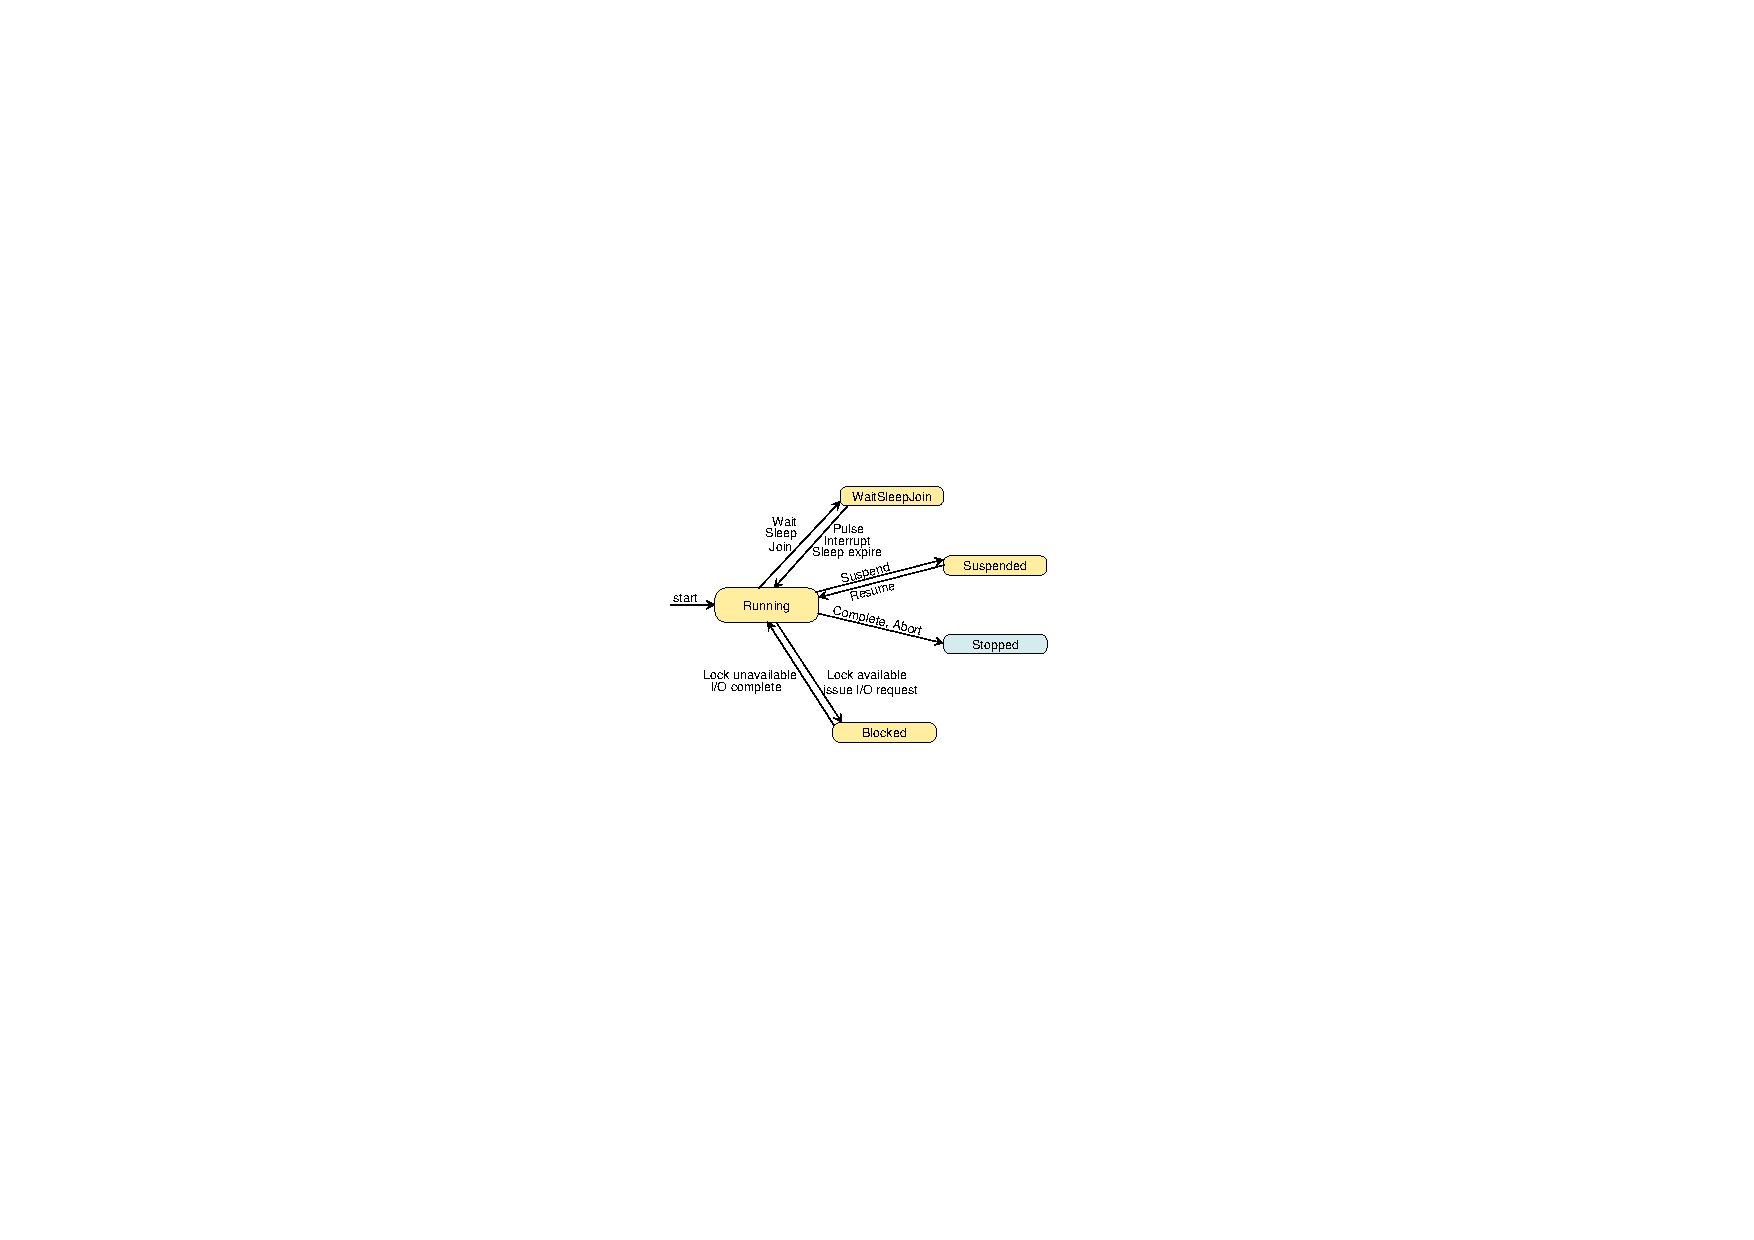
\includegraphics[width=\textwidth]{lib-thstate}
\end{figure}
\end{frame}

\begin{frame}
\frametitle{System.Threading 命名空间}
\begin{itemize}
\setlength{\itemsep}{6pt plus 1pt}
\item Thread 类用于创建和管理线程,设置优先级等
\item ThreadPool 类提供预先分配的线程池,可直接使用
\item Monitor 类负责线程的同步,实现对象的访问的机制
\item Mutex 实现一个同步基元,也可用于进程间同步
\item Semaphore 限制可同时访问某一资源的线程数
\item Timer 提供以指定的时间间隔执行方法的机制
\end{itemize}
\end{frame}

\begin{frame}[fragile]
\frametitle{Thread 类}
Thread 类的构造函数:
\begin{lstlisting}
public sealed class Thread
{
  public Thread(ThreadStart start);
  public Thread(ParameterizedThreadStart start);

  public Thread(ThreadStart start, int n);
  public Thread(ParameterizedThreadStart start, int n);
  // other members
}
public delegate void ThreadStart();
public delegate void ParameterizedThreadStart(object obj);
\end{lstlisting}

\begin{itemize}
\item ThreadStart --- 表示此线程开始执行时要调用的委托
\item ParameterizedThreadStart --- 同上,但可有一个参数
\item int n --- 限制线程堆栈大小的整数
\end{itemize}
\end{frame}

\begin{frame}[fragile]
\frametitle{线程的启动}
\begin{lstlisting}
public sealed class Thread
{
  ...
  public void Start();
  public void Start(object obj);

  // other memebers
}
\end{lstlisting}
\begin{itemize}
\item 线程创建后,需要通过 Start 方法开始线程的运行
\item 参数 obj 传给带参数的委托
\end{itemize}
\end{frame}

\begin{frame}[fragile]
\frametitle{创建并运行线程}
\begin{lstlisting}[escapeinside='']
using System;  using System.Threading;
public class ThreadExample {
  public static void ThreadProc() {
    for (int i = 0; i < 10; i++) {
      Console.WriteLine("ThreadProc: {0}", i);
      Thread.Sleep(0); }
  }
  public static void Main() {

    Thread t = new Thread(new ThreadStart(ThreadProc));
    t.Start(); // '线程开始运行'

    for (int i = 0; i < 4; i++) {
      Console.WriteLine("Main thread: Do some work.");
      Thread.Sleep(0);
    }
  }
}
\end{lstlisting}
\end{frame}

\begin{frame}[fragile]
\frametitle{给线程传递参数}
C\# 2.0 中,可以通过 ParameterizedThreadStart 委托给线程传递一个对象参数
\begin{lstlisting}
  public static void ThreadProc(object o) {
    for (int i = 0; i < (int)o; i++) {
      Console.WriteLine("ThreadProc: {0}", i);
      Thread.Sleep(0); }
  }
...
    Thread t = new Thread(ThreadProc);
    // new ParameterizedThreadStart(ThreadProc)

    t.Start(20);
...
\end{lstlisting}
\end{frame}

\begin{frame}[fragile]
\frametitle{Thread 类的成员特性}
\begin{lstlisting}
public sealed class Thread {
  public static Thread CurrentThread
  public int ManagedThreadId
  public string Name

  public ThreadPriority Priority
  public ThreadState ThreadState

  public bool IsAlive
  public bool IsBackground
  public bool IsThreadPoolThread
}
\end{lstlisting}
\begin{itemize}
\item CurrentThread --- 静态成员,获取当前正在运行的线程
\item Name --- 获取或设置线程的名称,只写一次
\item Priority --- 获取或设置一个值,该值指示线程的调度优先级
\item ThreadState --- 获取一个值,该值包含当前线程的状态
\end{itemize}
\end{frame}

% \begin{frame}
% \frametitle{Thread 类的成员方法}
% \begin{itemize}
% \item void Abort() --- 引发 ThreadAbortException,以开始终止此线程的过程
% \item void Interrupt() --- 中断处于 WaitSleepJoin 线程状态的线程
% \item void Join() --- 阻塞调用线程,直到某个线程终止为止
% \item bool Join(int/TimeSpan) --- 阻塞调用线程,直到某个线程终止或经过了指定时间为止
% \item static void Sleep(int/TimeSpan) --- 将当前线程挂起指定的时间
% \end{itemize}
% \end{frame}

\begin{frame}[fragile]
\frametitle{创建多个线程}
创建多个 Thread 实例即可:
\begin{lstlisting}[escapeinside='']
...
  public static void Main() {
    Thread t1 = new Thread(new ThreadStart(ThreadProc));
    Thread t2 = new Thread(ThreadProc)); //'自动转换'
    Thread t3 = new Thread(ThreadProc));

    t1.Start();
    t2.Start();
    t3.Start();

    for (int i = 0; i < 4; i++) {
      Console.WriteLine("Main thread: Do some work.");
      Thread.Sleep(0);
    }
  }
\end{lstlisting}
\end{frame}

\begin{frame}[fragile]
\frametitle{判断线程的结束}
通过读取 IsAlive 特性的值:
\lstset{emph={IsAlive}}
\begin{lstlisting}
  Thread t1, t2, t3; // new Thread(...)
  ...
  t1.Start(); t2.Start(); t3.Start();

  do {
    Console.WriteLine("Waiting thread");
    Thread.Sleep(100);
  } while (t1.IsAlive && t2.IsAlive && t3.IsAlive);

\end{lstlisting}
\end{frame}

\begin{frame}[fragile]
\frametitle{等待线程结束}
Thread 中定义的 Join 方法:
\begin{lstlisting}[escapeinside='']
public sealed class Thread {
  public void Join ();
  public bool Join (int ms);
  public bool Join (TimeSpan timeout);
  // '如果等待时间结束,则返回,值为 false'
}
\end{lstlisting}
\pause
使用 Join 等待线程结束,将进入 WaitSleepJoin 状态:
\lstset{emph={Join}}
\begin{lstlisting}
  Thread t1, t2, t3; // new Thread(...)
  ...
  t1.Start(); t2.Start(); t3.Start();

  t1.Join();  Console.WriteLine("Child #1 joined.");

  t2.Join();  Console.WriteLine("Child #2 joined.");

  t3.Join();  Console.WriteLine("Child #3 joined.");

\end{lstlisting}
\end{frame}

\begin{frame}[fragile]
\frametitle{挂起线程}
用于挂起 (\textit{suspend}) 和恢复 (\textit{resume}) 线程的两个方法: 
\begin{lstlisting}
public sealed class Thread{
  public void Resume();
  public void Suspend();
}
\end{lstlisting}
\begin{itemize}
\item 任何线程都可以挂起其他线程
\item 被挂起的线程只能被其他线程恢复
\item C\# 2.0 推荐使用其他方式暂停线程执行
\end{itemize}

\end{frame}


\begin{frame}[fragile]
\frametitle{使线程睡眠}
\begin{itemize}
\item Sleep 静态方法使线程睡眠,进入 WaitSleepJoin 状态
\end{itemize}
\begin{lstlisting}
public sealed class Thread {
  public static void Sleep (int ms);
  public static void Sleep (TimeSpan timeout);

  public static void SpinWait(int iterations);
}
\end{lstlisting}
\begin{itemize}
\item int 值表示毫秒数,为 0 时可用于线程切换
\item TimeSpan 可以方便的表示时间段
\begin{itemize}
\item TimeSpan.Infinite --- 无限
\item TimeSpan.FromDays(2) --- 2 天
\end{itemize}
\item SpinWait 导致线程等待由 iterations 参数定义的时间量
\end{itemize}
\end{frame}

\begin{frame}[fragile]
\frametitle{中止线程执行}
Thread 类的中止方法:
\begin{lstlisting}
public sealed class Thread {
  public void Abort();
  public void Abort(object stateInfo);
  public staic void ResetAbort();
}
\end{lstlisting}
\begin{itemize}
\item 被中止的线程会发生 ThreadAbortException 异常
\item 线程中的即使 catch 该异常,也会被中止,除非调用 Thread.ResetAbort()
\item 该异常的成员 ExceptionState 即 stateInfo 参数
\item WaitSleepJoin 状态的线程可被中止,但 Suspended 不可以
\end{itemize}
\end{frame}

\begin{frame}[fragile,plain]
\frametitle{线程中止的示例}
\lstset{emph={ExceptionState,Abort}}
\begin{lstlisting}
...
  public static void DoWork()
  { try
    { int i = 0;
      while (true) Console.WriteLine (i++);
    }
    catch (ThreadAbortException e)
    { string c ;
      c = (string) e.ExceptionState;
      Console.WriteLine (c);
    }
  }
  static void Main()
  {
    Thread w = new Thread (DoWork);
    w.Start();
    Thread.Sleep (200);
    w.Abort ("Time to go");
    w.Join();
  }
\end{lstlisting}
\end{frame}

\begin{frame}[fragile]
\frametitle{线程的优先级}
Thread 类中的优先级特性:
\begin{lstlisting}
public sealed class Thread {
  public ThreadPriority Priority {get; set};
}
public enum ThreadPriority {
  Lowest, BelowNormal, Normal, AboveNormal, Highest
}
\end{lstlisting}
\begin{itemize}
\item 高优先级得到更多的 CPU 时间
\item 具体调度算法随操作系统而不同
\end{itemize}
\begin{lstlisting}
  Thread t1, t2; // new Thread(...)
  ...
  t1.Priority = ThreadPriority.AboveNormal;
  t2.Priority = ThreadPriority.Normal;
  ...
  t1.Start(); t2.Start();
\end{lstlisting}
\end{frame}

\begin{frame}
\frametitle{线程同步}
\begin{block}{\textit{Synchronizing Threads}}
\CJKindent 确保多个线程对共享资源进行互斥访问的技术。
\end{block}
\begin{itemize}
\item 互斥锁(\textit{Mutex})
\item 信号量(\textit{Semaphore})
\item 临界区(\textit{Critical region})
\item 线程安全(\textit{Thread-safe})
\end{itemize}
\end{frame}

\begin{frame}[fragile]
\frametitle{线程同步}
% lock, Wait(), Pulse(), PulseAll()
\begin{itemize}
\item 当同一资源只能被一个线程使用时,需要使用同步技术
\item 使用 \texttt{lock} 进行同步非常容易
\item 也可以使用功能更全的 Monitor 类来实现
\end{itemize}
\medskip
\begin{itemize}
\item Monitor 类用于线程的同步
\item Mutex 和 Semaphore 类可用于线程和进程的同步
\end{itemize}
\end{frame}

\begin{frame}[fragile]
\frametitle{Monitor 类}
静态类 Monitor 中用于控制进入临界区的方法:
\begin{lstlisting}
public static class Monitor {
  public static void Enter(object obj);
  public static void Exit(object obj);
 
  public static bool TryEnter(object obj);
  public static bool TryEnter(object obj, int ms);
  // other members
}
\end{lstlisting}

\begin{itemize}
\item Monitor 类使用某个对象 obj 作为临界条件
\item Enter 方法如果得到 obj,进入临界区,否则被阻塞 (\textit{blocked})
\item Exit 方法释放 obj,退出临界区
\item TryEnter 如果没有得到 obj,不会被阻塞,但返回 \texttt{false}
\end{itemize}
\end{frame}

\begin{frame}[fragile]
\frametitle{使用 Monitor 同步示例}
\lstset{emph={Enter,Exit}}
\begin{lstlisting}
public class MyClass {
  public void DoSomething() 
  {...}
}
...
  MyClass obj = new MyClass();
  ...

  Monitor.Enter(obj);
  obj.DoSomething(); // thread-safe
  Monitor.Exit(obj);

\end{lstlisting}
\end{frame}

% \begin{frame}[fragile]
% \frametitle{保护静态成员}
% \begin{itemize}
% \item 静态成员是相应于类的,但所有对象都可以访问
% \item 针对对象的线程安全无法直接保护静态字段和方法
% \item 通过 \texttt{typeof} 操作符返回类的类型对象,作为临界条件
% \end{itemize}
% \lstset{emph={typeof}}
% \begin{lstlisting}
% public class MyClass{
%   static public void DoSomething();
%   {...}
% }
% ...
%   Monitor.Enter(typeof(MyClass));
%   MyClass.DoSomething();
%   Monitor.Exit(typeof(MyClass));
% \end{lstlisting}
% \end{frame}

\begin{frame}[fragile]
\frametitle{错误处理}
\begin{itemize}
\item 临界区内发生异常,如果没有释放临界条件就可能发生死锁
\item 要使用 \texttt{try/finally} 语句来避免
\end{itemize}
\lstset{emph={finally, Exit}}
\begin{lstlisting}
  Monitor.Enter(obj);
  try{
    obj.DoSomething();
  }
  // catch if needed
  finally{
    Monitor.Exit(obj);
  }
\end{lstlisting}
\end{frame}

\begin{frame}[fragile]
\frametitle{使用\texttt{lock} 简化Monitor}
\begin{itemize}
\item 编译器会将加锁语句(\texttt{lock}) 翻译为带有异常处理的 Monitor 语句
\end{itemize}
\begin{lstlisting}
  MyClass obj = new MyClass();
  ...
  // for objects
  lock(obj)
  {
    obj.DoSomething();
  }

  // for static memebers
  lock(typeof(MyClass))
  {
    MyClass.DoSomething();
  }
\end{lstlisting}
\end{frame}

\begin{frame}[fragile]
\frametitle{同时需要多个锁}
\begin{itemize}
\item 多个 \texttt{lock} 语句表示需要多个临界条件
\begin{lstlisting}
  MyClass obj1 = new MyClass();
  MyClass obj2 = new MyClass();
  MyClass obj3 = new MyClass();
  
  lock (obj1)
  lock (obj2)
  lock (obj3)
  {
    // Use the objects
  }
\end{lstlisting}
\item 如果线程间加锁顺序不同,会发生死锁
\item 需要多个锁,最好使用 \texttt{WaitHandle} 类
\end{itemize}
\end{frame}

\begin{frame}[fragile]
\frametitle{封装 Monitor}
\begin{itemize}
\item 在对象内部,使用 this 关键字可以对自己加锁
\end{itemize}
\lstset{emph={lock,this}}
\begin{lstlisting}
public class MyClass{
  public void DoSomething(){
    lock(this){
      //Do something
    }
  }
}
  MyClass obj = new MyClass();
  ...
  obj.DoSomething();  

\end{lstlisting}
\end{frame}

% \begin{frame}[fragile]
% \frametitle{Monitor 和泛型}
% \begin{lstlisting}
% public class MyClass<T>
% { T m_T;
%   public void SomeMethod() {
%     lock(this) {
%       // some thing here
%     }
%   }
% }
% \end{lstlisting}
% \begin{itemize}
% \item 如果想对类型参数加锁,需要限制为引用类型
% \end{itemize}
% \begin{lstlisting}
% public class MyClass<T> where T : class
% { ... }
% public class MyClass<T> where T : OtherClass
% { ... }
% \end{lstlisting}
% \end{frame}

\begin{frame}[fragile]
\frametitle{线程间的等待}
\begin{itemize}
\item 当得到锁后,又想暂停运行,需要暂时释放锁
\item 其他线程完成临界区任务后,需要通知暂停的线程
\item Monitor 中提供了如下方法:
\begin{lstlisting}
public static class Monitor {
  public static bool Wait(object obj);
  public static bool Wait(object obj, int ms);
  public static bool Wait(object obj, TimeSpan t);
  
  public static void Pulse(object obj);
  public static void PulseAll(object obj);
}
\end{lstlisting}
\end{itemize}

\end{frame}

\begin{frame}[fragile]
\frametitle{线程间的等待}
\begin{itemize}
\setlength{\itemsep}{6pt plus 1pt}
\item Wait 方法释放锁对象 obj,进入 WaitSleepJoin 状态等待通知
\item Pulse 方法通知 obj 对象的等待队列头的线程,锁对象状态即将改变;此时该线程将从 WaitSleepJoin
  状态变为 Blocked 状态,等待锁对象 obj 被释放
\item PulseAll 方法同上,但影响 obj 对象等待队列的所有线程
\item 只有锁的占有者才可以调用 Wait、Pulse 或 PulseAll 方法
\end{itemize}
\begin{columns}
\column{.5\textwidth}
\begin{lstlisting}
void Lock_Wait(object obj) {
  lock(obj){
    ... // Do some work
    Monitor.Wait(obj);
    ... // And some others
  }
}
\end{lstlisting}
\column{.5\textwidth}
\begin{lstlisting}
void Lock_Pulse(object obj) {
  lock(obj){
    ... // Do some work
    Monitor.Pulse(obj);
    ... // And some others
  }
}
\end{lstlisting}
\end{columns}
\end{frame}

\begin{frame}[fragile,plain]
\frametitle{等待示例}
\lstset{emph={Wait,Pulse,lock}}
\begin{lstlisting}[escapeinside='']
class MonitorSample {
  public Queue q = new Queue(); 
  public void run1() { // for thread 1
    int counter = 0;
    lock(q) {
      while(counter < 1000) {
        Monitor.Wait(q);    // '释放并等待'
        q.Enqueue(counter++);
        Monitor.Pulse(q); } // '通知'
    }
  }
  public void run2() { // for thread 2
    lock(q) {
      Monitor.Pulse(q);
      while(Monitor.Wait(q,1000)) {
        int counter = (int)q.Dequeue();
        Monitor.Pulse(q); } //end of while
    }
  }
}
\end{lstlisting}
\end{frame}

\begin{frame}[fragile,plain]
\frametitle{Mutex 类}
% http://msdn2.microsoft.com/zh-cn/library/system.threading.mutex.aspx
\begin{itemize}
\item 用于定义互斥锁(\textit{mutex})
\item 调用 WaitOne 方法获得锁,进入临界区,否则被阻塞
\item ReleaseMutex 方法用于释放锁
\end{itemize}

\begin{lstlisting}
public sealed class Mutex : WaitHandle{
  public Mutex();
  public Mutex(bool initOwned);
  public Mutex(bool initOwned, string name);
  public void ReleaseMutex();

  public static Mutex OpenExisting(string name);
  
  // other members
}

public abstract class WaitHandle{
  public virtual bool WaitOne();
  public virtual void Close();
  // other members  
}
\end{lstlisting}
\end{frame}

\begin{frame}[fragile]
\frametitle{Mutex 的使用}
\lstset{emph={WaitOne,ReleaseMutex}}
\begin{lstlisting}
public class MutexDemo: IDisposable {
  Mutex m = new Mutex();
  string s;
  public string Str
  { 
    set { 
      m.WaitOne();
      s = value;
      m.ReleaseMutex(); }

    get { 
      m.WaitOne();
      string temp = s;
      m.ReleaseMutex();
      return temp; } 
  }
  public void Dispose()
  { m.Close(); }
}
\end{lstlisting}
\end{frame}


\begin{frame}[fragile]
\frametitle{Semaphore 类}
% http://msdn2.microsoft.com/zh-cn/library/system.threading.semaphore.aspx
\begin{itemize}
\item C\# 2.0 的 Semaphore 类,用于限制访问临界资源的线程数
\item 初始化信号量时,可指定已占用的信号量和最大数量
\item Release 方法可以释放一个或多个信号量
\end{itemize}
\begin{lstlisting}
public sealed class Semaphore : WaitHandle {
  public Semaphore (int init, int max);
  public Semaphore (int init, int max, string name);
  public int Release();
  public int Release(int releaseCount);

  public static Semaphore OpenExisting(string name);
}
\end{lstlisting}
\end{frame}

\begin{frame}[fragile]
\frametitle{Interlocked 类}
\begin{itemize}
\item 静态类Interlocked 为多个线程共享的变量提供原子操作
\item 简化对单个变量访问的线程安全问题
\end{itemize}
\begin{lstlisting}[escapeinside='']
public static class Interlocked {
  public static int Increment(ref int loc);
  public static int Decrement(ref int loc);
  public static int Add(ref int loc, int val);

  public static int Exchange(ref int loc, int val);
  // other memebers for '\texttt{\bfseries double, float, long} \dots' 
}
\end{lstlisting}
\begin{itemize}
\item 例如,对静态变量的修改:
\lstset{emph={Interlocked,Increment}}
\begin{lstlisting}
public class SomeClass {
  public static int count = 0;
} ...
  Interlocked.Increment(ref SomeClass.count);
...
\end{lstlisting}
\end{itemize}
\end{frame}

\begin{frame}[fragile]
\frametitle{.NET 多线程服务}
\begin{itemize}
\item 线程相关的静态变量
\begin{lstlisting}
  [ThreadStatic]
  static string m_MyString;
\end{lstlisting}
\item 线程本地存储 TLS (\textit{Thread Local Storage})
\begin{lstlisting}
public sealed class Thread {
  public static LocalDataStoreSlot AllocateDataSlot();
  public static LocalDataStoreSlot 
                      AllocateNamedDataSlot(string n);
  public static LocalDataStoreSlot
                      GetNamedDataSlot(string name);
}
\end{lstlisting}
\item 线程池 (\textit{Thread Pool})
\end{itemize}
\end{frame}

\begin{frame}[fragile]
\frametitle{ThreadPool 类}
% http://msdn2.microsoft.com/zh-cn/library/0ka9477y.aspx
\begin{itemize}
\item 每个进程都有一个线程池,由 .NET 分配和管理
\item 线程池中的线程,不需要创建,可以直接使用
\item 通过静态类 ThreadPool 来使用线程池
\end{itemize}
\begin{lstlisting}
public static class ThreadPool{
  public static bool QueueUserWorkItem(WaitCallback c);
  public static bool
           QueueUserWorkItem(WaitCallback c, object s);
  // other memebers
}
public delegate void WaitCallback (Object s);
\end{lstlisting}
\end{frame}

\begin{frame}[fragile]
\frametitle{线程池的使用}
\begin{itemize}
\item 线程池线程也是线程对象,可以作为 Thread 对象使用
\item 线程池线程特性 IsThreadPoolThread 为 true
\end{itemize}
\lstset{emph={QueueUserWorkItem}}
\begin{lstlisting}
  void MyWork(object state){
    // check out
    Thread c = Thread.CurrentThread;
    Debug.Assert(c.IsThreadPooThread);
    int threadID = c.ManagedThreadId;
    Trace.WriteLine("Called on thread: " + threadID);

    // Do my work ...
  }

  ThreadPool.QueueUserWorkItem(MyWork);
\end{lstlisting}
\end{frame}


\begin{frame}[fragile]
\frametitle{Timer 类}
\begin{itemize}
\item Timer 类用于定时执行某一任务
\item Timer 类使用线程池线程
\end{itemize}
\begin{lstlisting}
public sealed class Timer {
  public Timer(TimerCallback callback,
               object state,
               long dueTime, 
               long period);

  public bool Change(int d, int p);

  public void Dispose();
}
public delegate void TimerCallback(object state);
\end{lstlisting}
\end{frame}

\begin{frame}[fragile]
\frametitle{Timer 的使用}
\begin{lstlisting}
using System;  using System.Threading;
class prog
{
  public static int counter = 0;
  public static Timer T;

  public static void run(object o)
  { Console.WriteLine (counter++); }

  static void Main()
  {
    T = new Timer (run, null, 0, 1000);
    Thread.Sleep (4000);
    T.Dispose(); T=null;
  }
}
\end{lstlisting}
\end{frame}

% Local Variables:
% mode: LaTeX
% TeX-master: "part-04.tex"
% TeX-header-end: "% End-of-Header$"
% TeX-trailer-start: "% Start-of-Trailer$"
% fill-column: 100
% coding: utf-8
% End:

